\subsubsection{Ward-management}

\begin{center}
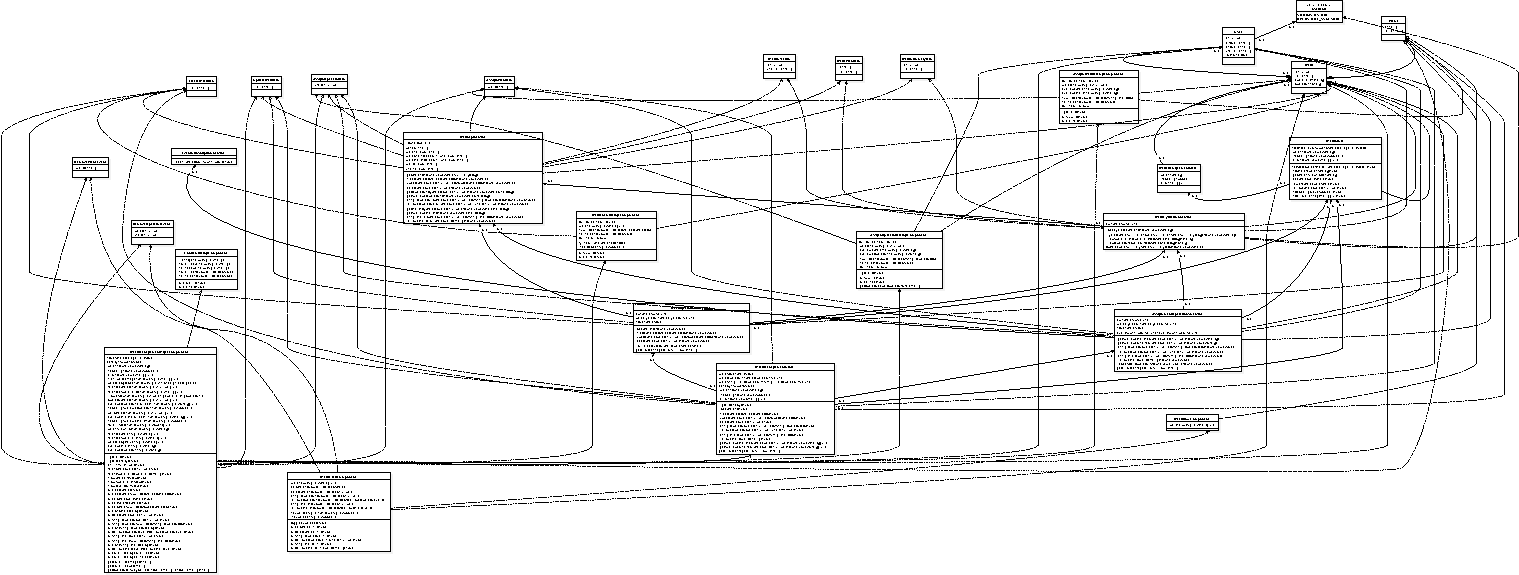
\includegraphics[width=\textwidth]{./frontend/ward-management/ward-management.pdf}
\captionof{figure}{\href{https://snakebyteteam.github.io/3-PB/Documenti_esterni/Specifica_tecnica/frontend/ward-management/ward-management.pdf}{Diagramma delle classi del modulo Ward management}}
\end{center}


\addAtr{-}{formBuilder: FormBuilder}{}
\addAtr{+}{wardId: input$<$number$>$}{}
\addAtr{+}{availableWards: input$<$Ward[]$>$}{}
\addAtr{+}{availableOperators: input$<$User[]$>$}{}
\addAtr{+}{submitted: output$<$AssignOperatorDto$>$}{}
\addAtr{+}{cancelled: output$<$void$>$}{}
\addAtr{+}{form: FormGroup}{}
\addMet{+}{ngOnInit() : void}{Inizializza il componente resettando lo stato del modulo reattivo per garantire un punto di partenza pulito a ogni apertura del dialogo.}
\addMet{+}{onSubmit() : void}{Valida i dati del modulo e, in caso di successo, emette l'evento di assegnazione con l'identificativo dell'operatore selezionato.}
\addMet{+}{onCancel() : void}{Notifica al componente genitore l'annullamento dell'operazione di assegnazione.}
\addMet{+}{getOperatorLabel(operator: User) : string}{Costruisce un'etichetta leggibile per l'operatore, privilegiando il nome completo rispetto allo username.}
\makeCl{AssignOperatorDialogComponent}{Componente che gestisce l'interfaccia di dialogo per l'assegnazione di un operatore sanitario a un reparto specifico. Utilizza i Reactive Forms di Angular per la gestione della selezione e della validazione dell'input utente.}

\addAtr{-}{formBuilder: FormBuilder}{}
\addAtr{+}{wardId: input$<$number$>$}{}
\addAtr{+}{availableWards: input$<$Ward[]$>$}{}
\addAtr{+}{availablePlants: input$<$Plant[]$>$}{}
\addAtr{+}{submitted: output$<$AssignPlantDto$>$}{}
\addAtr{+}{cancelled: output$<$void$>$}{}
\addAtr{+}{form: FormGroup}{}
\addMet{+}{ngOnInit() : void}{Inizializza lo stato del componente resettando il controllo del modulo reattivo dedicato alla selezione dell'impianto.}
\addMet{+}{onSubmit() : void}{Valida il modulo e, se i dati sono corretti, emette l'evento di sottomissione con l'identificativo dell'impianto (plantId) scelto per l'assegnazione al reparto.}
\addMet{+}{onCancel() : void}{Emette un segnale di annullamento per notificare la chiusura del dialogo senza apportare modifiche.}
\makeCl{AssignWardDialogComponent}{Componente che gestisce l'interfaccia di dialogo per l'assegnazione di un impianto a un determinato reparto. Sfrutta i Reactive Forms di Angular per gestire la logica di selezione e validazione dell'identificativo impianto.}

\addAtr{+}{ward: input$<$Ward $|$ null$>$}{}
\addAtr{+}{editWard: output$<$Ward$>$}{}
\addAtr{+}{deleteWard: output$<$number$>$}{}
\addAtr{+}{assignOperator: output$<$number$>$}{}
\addAtr{+}{removeOperator: output$<$RemoveOperatorEvent$>$}{}
\addAtr{+}{assignPlant: output$<$number$>$}{}
\addAtr{+}{removePlant: output$<$RemovePlantEvent$>$}{}
\addAtr{-}{isExpandedSignal: WritableSignal$<$boolean$>$}{}
\addAtr{+}{isExpanded: Signal$<$boolean$>$}{}
\addMet{+}{toggleExpanded() : void}{Inverte lo stato di espansione della scheda per mostrare o nascondere i dettagli aggiuntivi del reparto.}
\addMet{+}{onEditWardClick() : void}{Emette l'evento di modifica passando l'oggetto reparto corrente se presente.}
\addMet{+}{onDeleteWardClick() : void}{Invia l'identificativo del reparto per richiederne la rimozione dal sistema.}
\addMet{+}{onAssignOperatorClick() : void}{Sollecita l'apertura della logica di assegnazione di un nuovo operatore per il reparto attivo.}
\addMet{+}{onRemoveOperatorClick(userId: number) : void}{Emette un evento strutturato per dissociare uno specifico operatore sanitario dal reparto.}
\addMet{+}{onAssignPlantClick() : void}{Innesca la procedura per collegare un nuovo impianto tecnologico al reparto.}
\addMet{+}{onRemovePlantClick(plantId: string) : void}{Emette l'evento di rimozione dell'associazione tra l'impianto specificato e il reparto.}
\makeCl{WardCardComponent}{Componente di presentazione che visualizza le informazioni sintetiche di un reparto sotto forma di scheda espandibile. Coordina le interazioni dell'utente per la gestione del personale sanitario e degli impianti associati, delegando le operazioni di business tramite una serie di eventi in output.}

\addAtr{-}{formBuilder: FormBuilder}{}
\addAtr{+}{ward: input$<$Ward $|$ null$>$}{}
\addAtr{+}{submitted: output$<$CreateWardDto$>$}{}
\addAtr{+}{cancelled: output$<$void$>$}{}
\addAtr{+}{form: FormGroup}{}
\addAtr{-}{syncFormWithWard: Effect}{}
\addAtr{+}{isEditMode: Signal$<$boolean$>$}{}
\addMet{+}{onSubmit() : void}{Valida il contenuto del modulo e, in caso di successo, emette i dati del reparto (DTO) per la creazione o l'aggiornamento, applicando il trimming al nome.}
\addMet{+}{onCancel() : void}{Notifica la volontà dell'utente di chiudere il dialogo e annullare l'inserimento o la modifica dei dati.}
\makeCl{WardFormDialogComponent}{Componente di interfaccia per la creazione e la modifica dei reparti. Utilizza un approccio reattivo basato su \textbf{Signals} ed \textbf{Effects} per sincronizzare automaticamente i dati del modulo con l'input esterno, gestendo dinamicamente lo stato di editing e le regole di validazione del nome.}

\addAtr{-}{store: WardManagementStore}{}
\addAtr{-}{destroy\$: Subject$<$void$>$}{}
\addAtr{+}{wards\$: Observable$<$Ward[]$>$}{}
\addAtr{+}{isLoading\$: Observable$<$boolean$>$}{}
\addAtr{+}{error\$: Observable$<$string $|$ null$>$}{}
\addAtr{+}{snackbarMessage: WritableSignal$<$string $|$ null$>$}{}
\addAtr{+}{wardDialogMode: WritableSignal$<$'closed' $|$ 'create' $|$ 'edit'$>$}{}
\addAtr{+}{selectedWardId: WritableSignal$<$number $|$ null$>$}{}
\addAtr{+}{selectedWard: Signal$<$Ward $|$ null$>$}{}
\addAtr{+}{confirmState: WritableSignal$<$ConfirmState $|$ null$>$}{}
\addMet{+}{ngOnInit() : void}{Inizializza il componente caricando i reparti dallo store e sottoscrivendo gli stream per aggiornare lo stato locale e la gestione degli errori.}
\addMet{+}{selectWard(wardId: number) : void}{Gestisce la selezione di un reparto, aggiornando la vista e resettando la selezione degli appartamenti correlati.}
\addMet{+}{onCreateWardSubmit(dto: CreateWardDto) : void}{Invia la richiesta di creazione di un nuovo reparto allo store e chiude la finestra di dialogo.}
\addMet{+}{onAssignOperator(wardId: number) : void}{Avvia il processo di assegnazione operatore, recuperando la lista degli utenti disponibili per lo specifico reparto.}
\addMet{+}{onAssignPlantSubmit(dto: AssignPlantDto) : void}{Finalizza l'associazione di un impianto al reparto selezionato tramite lo store.}
\addMet{+}{onConfirmDialogConfirmed() : void}{Esegue l'azione di business (cancellazione reparto o rimozione associazione) basandosi sulla tipologia di conferma attiva.}
\addMet{+}{getConfirmMessage() : string}{Restituisce un messaggio testuale contestualizzato per il dialogo di conferma in base all'operazione che l'utente sta eseguendo.}
\makeCl{WardManagementPageComponent}{Componente "Smart" che funge da pagina principale per la gestione dei reparti. Coordina l'interazione tra lo store dei dati e i vari componenti di dialogo (creazione, assegnazione operatori, impianti), gestendo inoltre la navigazione a step per i dispositivi mobili e il feedback utente tramite snackbar.}

\addAtr{+}{plant: input$<$Plant $|$ null$>$}{}
\makeCl{WardRowComponent}{Componente di presentazione granulare utilizzato per visualizzare i dettagli di un singolo impianto (appartamento) all'interno della lista di un reparto. Riceve i dati tramite un input reattivo e adotta la strategia di \textbf{OnPush} per ottimizzare le prestazioni di rendering.}

\addAtr{+}{id: number}{}
\addAtr{+}{name: string}{}
\addAtr{+}{apartments: Plant[]}{}
\addAtr{+}{operators: User[]}{}
\makeAbCl{Ward}{Questa interfaccia definisce il modello dati di un reparto all'interno del sistema. Rappresenta l'entità organizzativa principale, collegando un identificativo unico e un nome a collezioni di impianti (appartamenti) e operatori sanitari assegnati.}

\addAtr{+}{id: string}{}
\addAtr{+}{name: string}{}
\makeAbCl{Plant}{Questa interfaccia definisce il modello dati di un impianto (spesso riferito a un appartamento) all'interno del sistema. Rappresenta l'unità tecnologica fondamentale, identificata da un codice univoco e un nome descrittivo, che viene associata ai reparti per il monitoraggio.}

\addAtr{+}{name: string}{}
\makeAbCl{CreateWardDto}{Data Transfer Object utilizzato per l'invio dei dati necessari alla creazione di un nuovo reparto, contenente esclusivamente il nome descrittivo.}

\addAtr{+}{name: string}{}
\makeAbCl{UpdateWardDto}{Data Transfer Object per l'aggiornamento delle informazioni di un reparto esistente.}

\addAtr{+}{userId: number}{}
\makeAbCl{AssignOperatorDto}{Oggetto per il trasferimento dei dati relativi all'associazione di un operatore sanitario a un reparto tramite il suo identificativo utente.}

\addAtr{+}{plantId: string}{}
\makeAbCl{AssignPlantDto}{Oggetto per il trasferimento dei dati relativi al collegamento di un impianto a un reparto tramite l'identificativo dell'impianto.}

\addAtr{+}{id: number}{}
\addAtr{+}{username: string}{}
\makeAbCl{WardUserDto}{Rappresentazione semplificata di un utente all'interno del contesto di gestione reparti, focalizzata su ID e nome utente.}

\addAtr{+}{id: string}{}
\addAtr{+}{name: string}{}
\makeAbCl{WardPlantDto}{Rappresentazione sintetica di un impianto associato a un reparto, utilizzata per il trasferimento dati tra client e server.}

\addAtr{+}{id: number}{}
\addAtr{+}{name: string}{}
\makeAbCl{WardSummaryDto}{Modello dati minimale che fornisce un riepilogo delle informazioni essenziali di un reparto.}

\addAtr{+}{wards: Ward[]}{}
\addAtr{+}{isLoading: boolean}{}
\addAtr{+}{error: string | null}{}
\makeAbCl{WardManagementState}{Interfaccia che definisce lo stato globale del modulo di gestione reparti, includendo la lista dei reparti, lo stato di caricamento e la gestione degli errori.}

\addAtr{+}{wardId: number}{}
\addAtr{+}{userId: number}{}
\makeAbCl{RemoveOperatorEvent}{Interfaccia che definisce la struttura dell'evento di rimozione di un operatore, specificando le chiavi esterne del reparto e dell'utente.}

\addAtr{+}{plantId: string}{}
\makeAbCl{RemovePlantEvent}{Interfaccia per l'evento di rimozione di un impianto, contenente l'identificativo univoco dell'asset da dissociare.}

\addAtr{-}{api: WardApiService}{}
\addAtr{-}{wardHydration: WardHydrationService}{}
\addAtr{-}{store: WardStore}{}
\addAtr{-}{eventSubscriptionService: EventSubscriptionService | null}{}
\addMet{+}{getAvailablePlantsForWard(wardId: number) : Observable$<$Plant[]$>$}{Recupera gli impianti disponibili filtrando quelli già assegnati ad altri reparti e ne esegue l'idratazione dei dati.}
\addMet{+}{getAvailableUsersForWard(wardId: number) : Observable$<$User[]$>$}{Fornisce l'elenco degli operatori che possono essere assegnati a un reparto, escludendo quelli già presenti nel reparto specificato.}
\addMet{+}{assignOperator(wardId: number, dto: AssignOperatorDto) : Observable$<$void$>$}{Esegue l'associazione di un operatore a un reparto e innesca il ricaricamento dello stato.}
\addMet{+}{removeOperator(wardId: number, userId: number) : Observable$<$void$>$}{Rimuove l'associazione di un operatore e aggiorna i dati sincronizzati nel sistema.}
\addMet{+}{assignPlant(wardId: number, dto: AssignPlantDto) : Observable$<$void$>$}{Assegna un impianto tecnologico a un reparto, gestendo la successiva propagazione degli aggiornamenti nello store.}
\addMet{+}{removePlant(plantId: string) : Observable$<$void$>$}{Dissocia un impianto dal relativo reparto e aggiorna le sottoscrizioni agli eventi di allarme.}
\addMet{-}{reloadAfter(operation\$: Observable$<$void$>$) : Observable$<$void$>$}{Metodo di utilità che incapsula la logica di post-esecuzione: ricarica i reparti idratati, aggiorna lo store globale e rinfresca le sottoscrizioni agli eventi.}
\makeCl{AssignmentOperationsService}{Servizio di dominio preposto alla gestione delle relazioni tra reparti, operatori e impianti. Centralizza la logica di assegnazione e rimozione delle risorse, garantendo che lo stato dell'applicazione e le sottoscrizioni agli eventi (WebSocket) rimangano sincronizzati con i cambiamenti effettuati sul backend.}

\addAtr{-}{http: HttpClient}{}
\addAtr{-}{baseUrl: string}{}
\addMet{+}{getWards() : Observable$<$WardSummaryDto[]$>$}{Recupera la lista sintetica di tutti i reparti censiti nel sistema.}
\addMet{+}{createWard(dto: CreateWardDto) : Observable$<$Ward$>$}{Invia una richiesta POST per la creazione di un nuovo reparto.}
\addMet{+}{updateWard(wardId: number, dto: UpdateWardDto) : Observable$<$Ward$>$}{Aggiorna i dati di un reparto esistente tramite una chiamata PUT.}
\addMet{+}{deleteWard(wardId: number) : Observable$<$void$>$}{Elimina definitivamente un reparto dal sistema.}
\addMet{+}{getOperatorsByWardId(wardId: number) : Observable$<$WardUserDto[]$>$}{Ottiene l'elenco dei soli operatori associati a uno specifico reparto.}
\addMet{+}{getAvailableOperators() : Observable$<$WardUserDto[]$>$}{Recupera la lista globale di tutti gli utenti/operatori potenzialmente assegnabili.}
\addMet{+}{assignOperatorToWard(wardId: number, dto: AssignOperatorDto) : Observable$<$void$>$}{Crea una nuova relazione nel database tra un reparto e un operatore.}
\addMet{+}{removeOperatorFromWard(wardId: number, userId: number) : Observable$<$void$>$}{Rimuove il legame associativo tra un reparto e un operatore specifico.}
\addMet{+}{getPlantsByWardId(wardId: number) : Observable$<$WardPlantDto[]$>$}{Recupera gli impianti (plant) attualmente collegati a un determinato reparto.}
\addMet{+}{getAvailablePlants() : Observable$<$WardPlantDto[]$>$}{Interroga il sistema per ottenere la lista completa di tutti gli impianti disponibili.}
\addMet{+}{assignPlantToWard(wardId: number, dto: AssignPlantDto) : Observable$<$void$>$}{Stabilisce un'associazione formale tra un reparto e un impianto tecnologico.}
\addMet{+}{removePlantFromWard(plantId: string) : Observable$<$void$>$}{Rimuove l'associazione di un impianto, svincolandolo dal reparto di appartenenza.}
\makeCl{WardApiService}{Servizio di comunicazione dati di basso livello che incapsula tutte le chiamate HTTP verso le API REST dedicate alla gestione dei reparti (Wards). Gestisce le operazioni CRUD e le relazioni molti-a-molti con operatori e impianti, garantendo la corretta formattazione degli URL e la gestione dei parametri tramite encodeURIComponent.}

\addAtr{-}{api: WardApiService}{}
\addMet{+}{loadHydratedWards() : Observable$<$Ward[]$>$}{Innesca il processo di caricamento completo dei reparti, recuperando prima le sintesi e poi arricchendo ogni elemento con i dati di dettaglio.}
\addMet{+}{hydrateWardSummaries(wardSummaries: WardSummaryDto[]) : Observable$<$Ward[]$>$}{Coordina la risoluzione parallela delle dipendenze per una lista di riepiloghi reparti utilizzando \textbf{forkJoin} per gestire le richieste asincrone simultanee.}
\addMet{+}{mapApartments(apartmentsDto: WardPlantDto[]) : Plant[]}{Esegue la mappatura strutturale tra i DTO degli impianti provenienti dal backend e il modello dati interno dell'applicazione.}
\addMet{+}{mapOperators(operatorsDto: WardUserDto[]) : User[]}{Trasforma i dati sintetici degli utenti in oggetti operatore completi, assegnando ruoli predefiniti e normalizzando i campi anagrafici.}
\addMet{-}{toWard(wardSummary: WardSummaryDto) : Observable$<$Ward$>$}{Metodo privato che aggrega le chiamate API per impianti e operatori di un singolo reparto, componendo l'oggetto di dominio finale \textbf{Ward}.}
\makeCl{WardHydrationService}{Servizio di orchestrazione responsabile del processo di "idratazione" dei dati. Il suo compito principale è trasformare oggetti DTO parziali in entità di dominio complete, aggregando informazioni provenienti da endpoint diversi (reparti, relazioni utenti, relazioni impianti) per fornire una vista coerente e pronta all'uso per l'interfaccia utente.}

\addAtr{-}{wardStore: WardStore}{}
\addAtr{-}{wardOperations: WardOperationsService}{}
\addAtr{-}{wardAssignmentOperations: AssignmentOperationsService}{}
\addAtr{-}{destroy\$: Subject$<$void$>$}{}
\addAtr{+}{wards\$: Observable$<$Ward[]$>$}{}
\addAtr{+}{isLoading\$: Observable$<$boolean$>$}{}
\addAtr{+}{error\$: Observable$<$string $|$ null$>$}{}
\addMet{+}{ngOnDestroy() : void}{Gestisce la pulizia delle sottoscrizioni attive tramite l'emissione del segnale sul Subject di distruzione.}
\addMet{+}{loadWards() : void}{Innesca il caricamento dei reparti aggiornando lo stato di loading e gestendo la sottoscrizione allo stream operativo.}
\addMet{+}{createWard(dto: CreateWardDto) : void}{Coordina la creazione di un nuovo reparto delegando l'operazione al servizio dedicato.}
\addMet{+}{updateWard(wardId: number, dto: UpdateWardDto) : void}{Gestisce l'aggiornamento dei dati di un reparto esistente.}
\addMet{+}{deleteWard(wardId: number) : void}{Esegue la rimozione di un reparto dal sistema.}
\addMet{+}{assignOperator(wardId: number, dto: AssignOperatorDto) : void}{Avvia la procedura di associazione di un operatore sanitario a un reparto.}
\addMet{+}{removeOperator(wardId: number, userId: number) : void}{Gestisce la dissociazione di un operatore da un reparto.}
\addMet{+}{assignPlant(wardId: number, dto: AssignPlantDto) : void}{Innesca l'assegnazione di un impianto tecnologico a un reparto specifico.}
\addMet{+}{removePlant(plantId: string) : void}{Esegue la rimozione di un impianto dal reparto a cui è associato.}
\addMet{+}{getAvailablePlantsForWard(wardId: number) : Observable$<$Plant[] $|$ null$>$}{Recupera gli impianti disponibili per l'assegnazione, gestendo eventuali errori di recupero dati.}
\addMet{+}{getAvailableUsersForWard(wardId: number) : Observable$<$User[] $|$ null$>$}{Recupera l'elenco degli utenti assegnabili al reparto, fornendo una gestione degli errori integrata.}
\makeCl{WardManagementStore}{Classe Facade che funge da punto di ingresso unico per la gestione dello stato e delle operazioni del modulo reparti. Coordina l'interazione tra i servizi operativi (WardOperations, AssignmentOperations) e lo storage dei dati (WardStore), esponendo stream reattivi per l'interfaccia utente e gestendo il ciclo di vita delle operazioni asincrone.}

\addAtr{-}{api: WardApiService}{}
\addAtr{-}{wardHydration: WardHydrationService}{}
\addAtr{-}{store: WardStore}{}
\addMet{+}{loadWards() : Observable$<$void$>$}{Innesca il caricamento asincrono dei reparti idratati, aggiornando lo store globale e gestendo eventuali errori di rete o di parsing.}
\addMet{+}{createWard(dto: CreateWardDto) : Observable$<$void$>$}{Invia la richiesta di creazione di un nuovo reparto; gestisce specificamente l'errore di conflitto (409) in caso di nome duplicato e aggiorna lo store con l'entità normalizzata.}
\addMet{+}{updateWard(wardId: number, dto: UpdateWardDto) : Observable$<$void$>$}{Esegue l'aggiornamento dei dati anagrafici di un reparto e sostituisce la versione precedente nello store mantenendo l'integrità delle relazioni esistenti.}
\addMet{+}{deleteWard(wardId: number) : Observable$<$void$>$}{Rimuove un reparto dal sistema tramite API e aggiorna coerentemente lo stato locale eliminando l'entità corrispondente.}
\addMet{-}{normalizeMutationWard(ward: Ward) : Ward}{Assicura che, a seguito di una mutazione (creazione o modifica), l'oggetto reparto mantenga le liste di appartamenti e operatori recuperandole dallo stato corrente se non fornite dal server.}
\addMet{-}{getErrorMessage(error: unknown) : string}{Analizza l'eccezione catturata per estrarre un messaggio di errore leggibile, privilegiando il contenuto della risposta HTTP o il messaggio di sistema.}
\makeCl{WardOperationsService}{Servizio operativo di dominio che orchestra le operazioni CRUD sui reparti. Funge da ponte tra i servizi di comunicazione (API), i servizi di trasformazione (Hydration) e la gestione dello stato (Store), garantendo che ogni transazione sui dati sia riflessa correttamente nell'interfaccia utente.}

\addAtr{-}{state\$: BehaviorSubject$<$WardManagementState$>$}{}
\addAtr{+}{wards\$: Observable$<$Ward[]$>$}{}
\addAtr{+}{isLoading\$: Observable$<$boolean$>$}{}
\addAtr{+}{error\$: Observable$<$string $|$ null$>$}{}
\addMet{-}{setState(partial: Partial$<$WardManagementState$>$) : void}{Metodo privato per l'aggiornamento atomico dello stato locale, garantendo l'immutabilità tramite la sovrascrittura selettiva delle proprietà.}
\addMet{+}{setWards(wards: Ward[]) : void}{Sovrascrive l'intera collezione dei reparti nello stato corrente.}
\addMet{+}{getWardsSnapshot() : Ward[]}{Restituisce il valore sincronizzato attuale della lista reparti senza attivare una sottoscrizione allo stream.}
\addMet{+}{addWard(ward: Ward) : void}{Aggiunge un nuovo reparto alla collezione esistente e resetta contemporaneamente gli indicatori di caricamento ed errore.}
\addMet{+}{replaceWard(ward: Ward) : void}{Aggiorna un reparto specifico all'interno della lista, mappando l'ID fornito con quello esistente per sostituirne i dati.}
\addMet{+}{removeWard(wardId: number) : void}{Elimina un reparto dallo stato filtrando la collezione in base all'identificativo fornito.}
\addMet{+}{setLoading(value: boolean) : void}{Aggiorna lo stato di attesa dell'interfaccia durante le operazioni asincrone.}
\addMet{+}{setError(message: string | null) : void}{Configura il messaggio di errore da visualizzare all'utente, forzando la disattivazione dello stato di caricamento.}
\makeCl{WardStore}{Classe di gestione dello stato a basso livello (Data Store) basata sul pattern \textbf{BehaviorSubject}. Funge da "Single Source of Truth" locale per il modulo dei reparti, esponendo flussi di dati reattivi e immutabili per garantire la coerenza della UI durante le operazioni di manipolazione dei dati.}